\chapter{Negative friction coefficient}\label{chap:negative_coef}
For the final part of this thesis, we concern ourselves with a proof of concept approach for the designing of a negative friction coefficient. From the pilot study (\cref{chap:pilot_study}) we found the friction of the two investigated Kirigami patterns to have a non-linear relationship with strain. This is hypothesized to yield a negative friction coefficient for certain load ranges in a coupled system of load and strain. We will investigate this hypothesis further in this chapter.

\section{Nanomachine coupling}
We do not attempt to simulate the dynamics of any nanomachine designs, but we propose that coupling between load and strain could be achieved, for instance, by following a design as sketched in~\cref{fig:nanomachine}. Such a design could perhaps be achieved by rigging carbon nanotubes in a similar configuration. 

\begin{figure}[H]
  \centering
  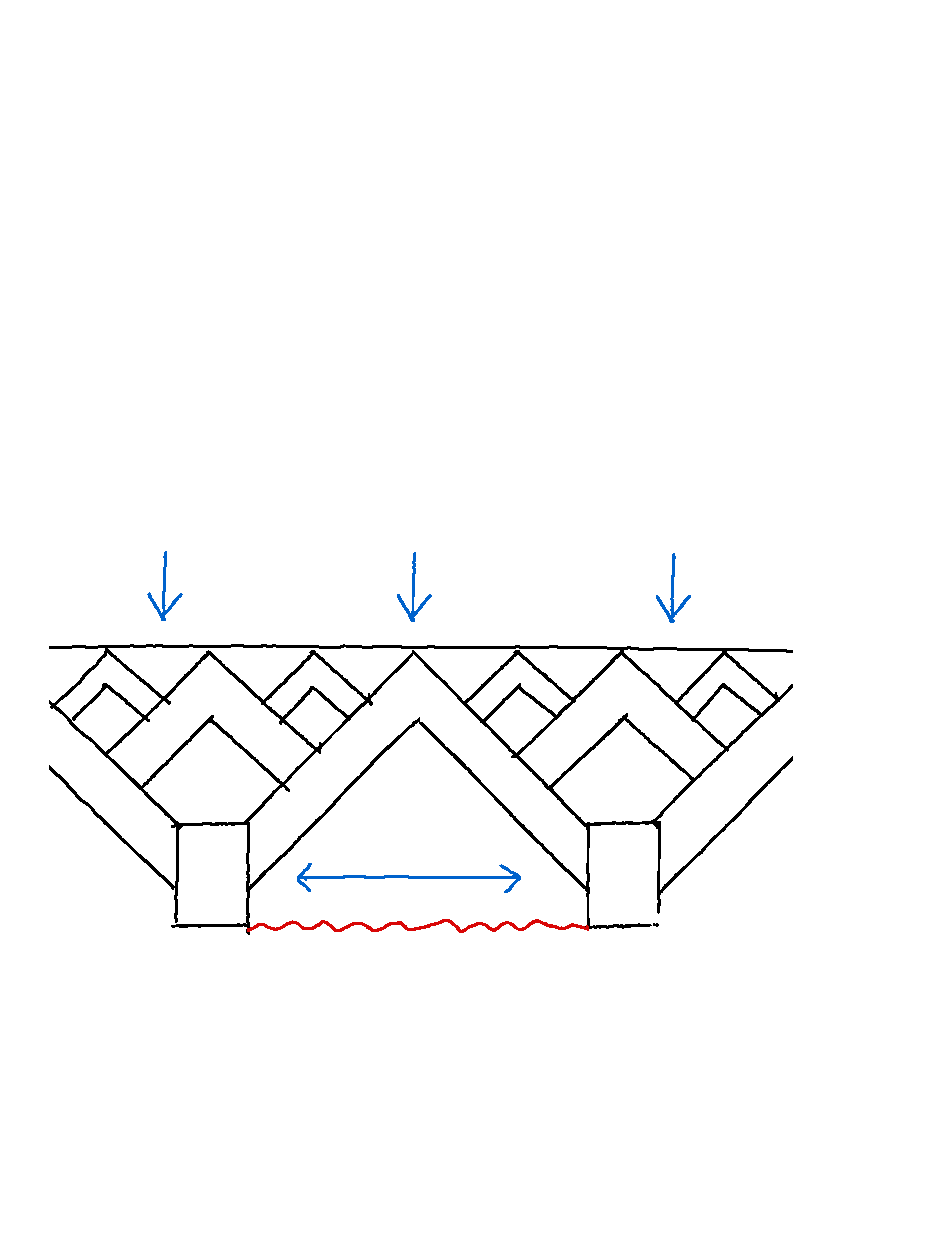
\includegraphics[width=0.5\linewidth]{figures/negative_coefficient/nanomachine.pdf}
  \caption{Working sketch for a nanomachine design that aims to translate applied load (from the top of the figure) to a straining of the graphene sheet (shown in red). The black boxes connected to the graphene sheet represent the pull blocks in our system.}
  \label{fig:nanomachine}
\end{figure}

We mimic the nanomachine coupling by implementing a load-depending tension force to our \acrshort{MD} simulations. So far, we have kept the pull block spaced by a fixed distance throughout the simulations, but now we let the pull blocks move relative to each other under the influence of tension. We let the tension force act in the $\pm y$ direction for each pull block respectively such that the force acts inwards toward the sheet. The magnitude of the tension force $F_t$ is modeled as a linear coupling to normal load $F_t = TF_N$ by a factor $T$ which represents the ratio for the load-to-strain coupling. We find that a ratio of
$T=6$ will provide the necessary tension for achieving a full strain range (till rupture) within the loading range used so far in our study. Notice that this coupling scheme is slightly different than that proposed in~\cref{eq:mu_strain} where we assumed a direct coupling between load and strain $\varepsilon = R F_N$. This modification provides a more standardized description of the proposed nanomachine since the relation between tension and strain will depend on the specific Kirigami sheet. We use the Tetrahedron
$(7,5,1)$ and Honeycomb $(2,2,1,5)$ from the pilot study and perform multiple
simulations for different normal loads. We use 100 uniformly spaced normal force
values in the range $[0, 15]$ nN which corresponds to a tension force of $[0, 90]$ nN. For the Tetrahedron pattern, we increase the load by a speed of \SI{0.015}{nN/ps}. Due to a rapid change in the strain-tension curve for the Honeycomb pattern, we reduced the loading speed to \SI{0.0015}{nN/ps} and added additional data points to the sparsely populated strain range. We compare the results to the pilot study results~\cref{fig:multi_stretch} by mapping the strain to load values corresponding to the strain-load curves found in the coupled system. The results are shown in~\cref{fig:negfric}.


\begin{figure}[!htb]
  \centering
  \begin{subfigure}[t]{\textwidth}
      \centering
      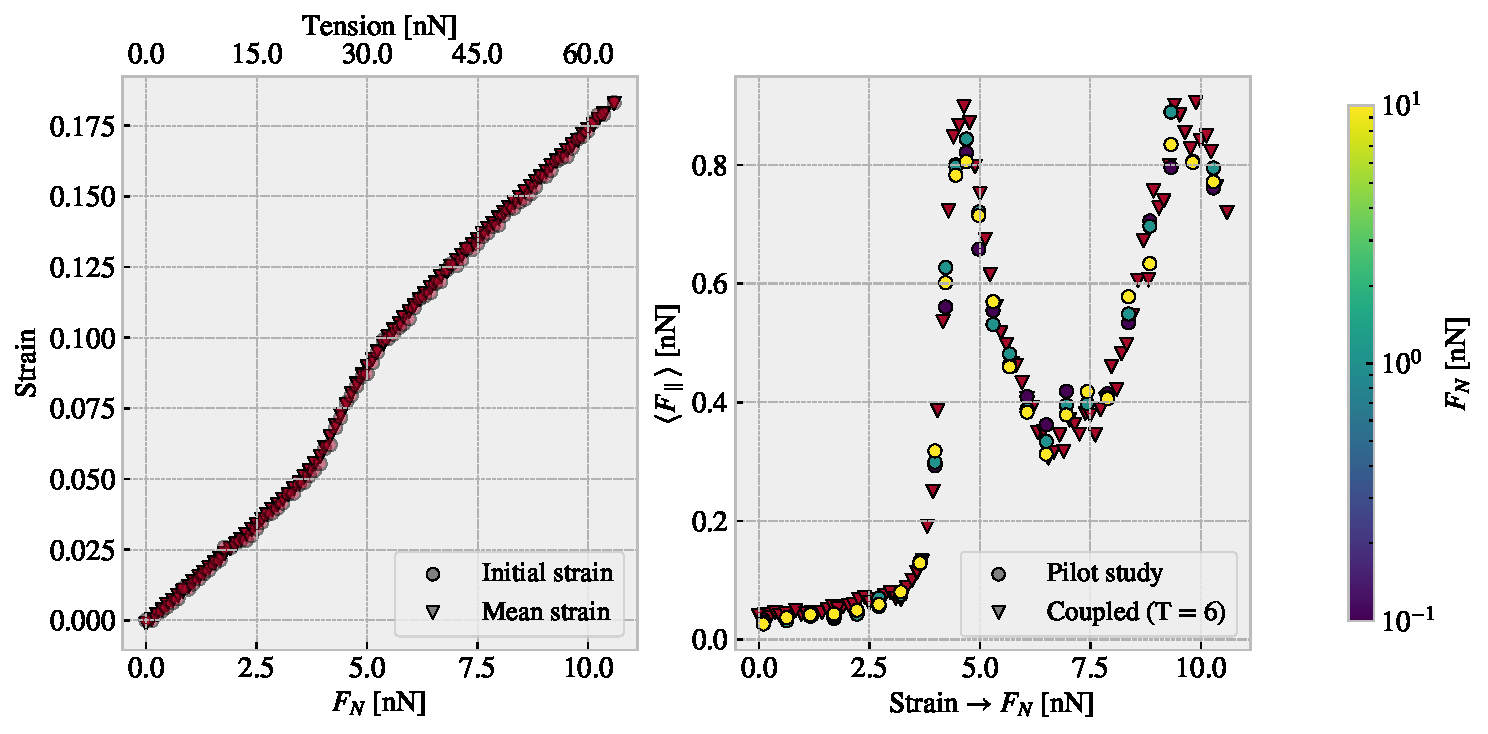
\includegraphics[width=\textwidth]{figures/negative_coefficient/manual_coupling_tension_pop7_5_1.pdf}
      \caption{Tetrahedron $(7,5,1)$}
      % \label{fig:}
  \end{subfigure}
  % \hfill
  \begin{subfigure}[t]{\textwidth}
    \centering
    \raggedleft
    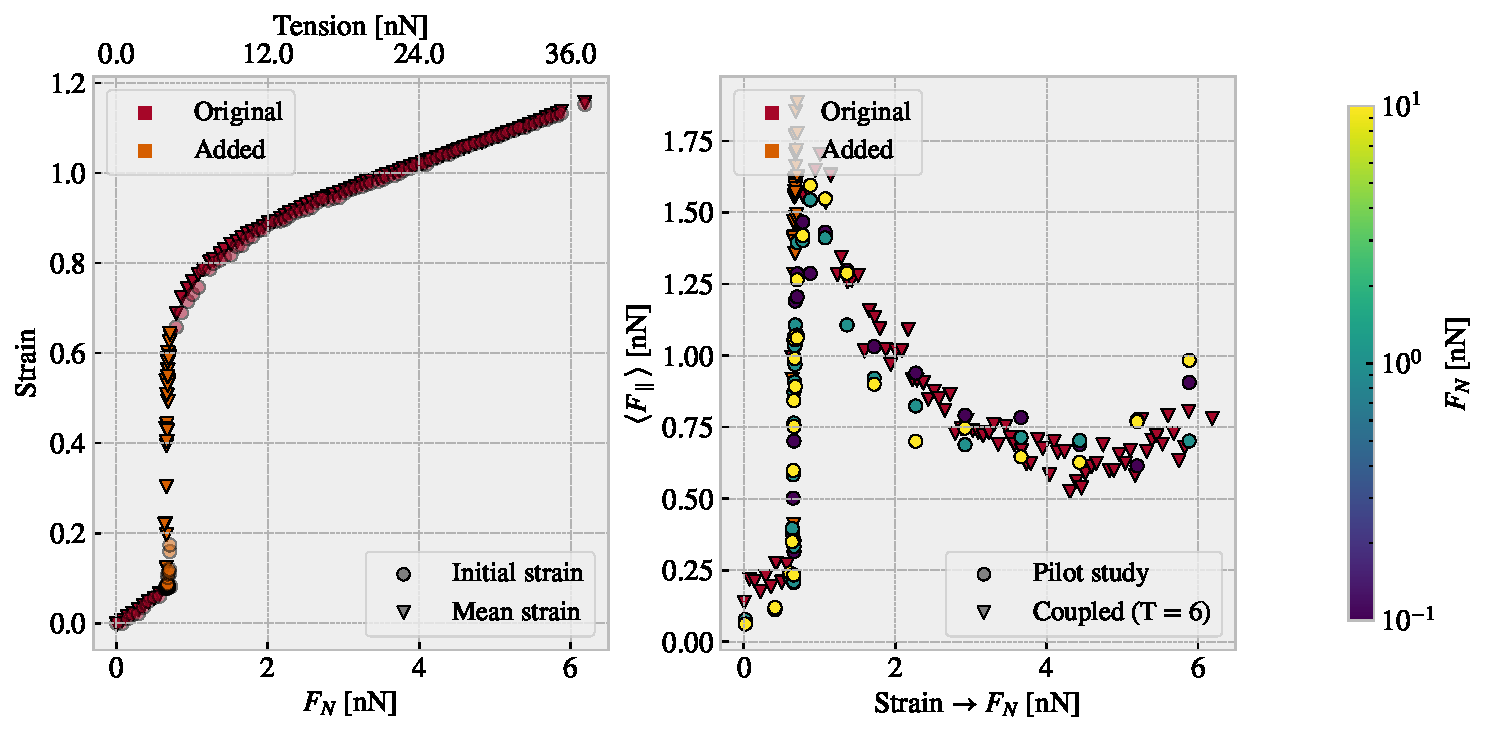
\includegraphics[width=0.98\textwidth]{figures/negative_coefficient/manual_coupling_tension_hon2215.pdf}
    \caption{Honeycomb $(2,2,1,5)$}
    % \label{fig:}
  \end{subfigure}
  \hfill
  \caption{Investigation of the friction response for a coupled system using (a)
  the Tetrahedron $(7,5,1)$ and (b) the Honeycomb $(2,2,1,5)$ pattern from the
  pilot study. The pull blocks are allowed to move relative to each other under
  the influence of a tension force $F_t$ modeled as $F_t = TF_N$ for normal load
  $F_N$ and a load-to-tension ratio $T=6$. The right panel shows the
  friction-load curve for the coupled system (orange and red triangles) in
  comparison to the results from the pilot study where the pull blocks are
  locked at a fixed separation distance and with a constant normal load
  (\cref{fig:multi_stretch}). The pilot study results have their strain values
  mapped to the normal load axis through the observed strain-load curve for the
  coupled system. Their original normal loads are indicated via the colors in
  the colorbar. The left panel shows the strain-tension curve. The circles
  denote the initial strain, at the beginning of the simulation, while the
  triangles denote the mean strain for the whole simulation. For the Honeycomb
  pattern, we have added more data points in the region where the strain-tension
  curve changed rapidly.}
  \label{fig:negfric}
\end{figure}

Generally, we observe from~\cref{fig:negfric} that the data points of the
coupled system align reasonably well with the mapped data points from the pilot
study. This indicates that the simultaneous loading and straining of the system
does not suppress the underlying mechanism governing the non-linear trends. For
the Tetrahedron pattern, we find an almost linear strain-tension curve which
makes for a recognizable trend in the friction-load curve similar to that seen
in the friction-strain curve in~\cref{fig:multi_stretch}. In both cases, we
also notice that the initial and the mean strains align rather well. This
suggests that the sliding does not contribute to a significantly increased
tension in the sheet which would otherwise lead to an increased strain as well.For the Honeycomb pattern, we find an interesting trend for the strain-tension
curve. At low tension, the curve of the strain is increasing seemingly linearly
with strain, but a drastic increase in strain happens at a tension of \SI{4.5}{nN} ($F_N = \SI{0.75}{nN}$) transitioning from a strain of roughly 0.08 to 0.7. Eventually, this settles off into a linear trend before reaching the rupture point. This
reflects the reason for decreasing the loading speed and adding more data points
to fill this gap in the strain-tension curve. The rapid increase in the strain-load
the curve makes for a similar rapid increase in the friction-load curve as well.
Hence we find that the Honeycomb coupled system essentially exhibits an initial discontinuous increase in friction with load, which is then followed by a longer region of decreasing friction with load. When considering the simulation frames in
\cref{sec:sheet_stretch} we notice that the strain range covered in this transition aligns rather well with the unfolding of the honeycomb pattern. As we have previously noted, the Honeycomb pattern unfolds in segments, with one segment buckling at a time. We observe that this unfolding is initiated after passing a minimum tension. During the unfolding phase, we observe an increase in friction, which is immediately followed by a decrease in friction with further straining. This suggests that exploring this mechanical transition further could be beneficial for gaining a deeper understanding of the underlying mechanisms involved. 

From the results in~\cref{fig:negfric} we have found that our proposed coupled system, based on a $T = 6$ load-to-tension coupling, demonstrates a significant negative friction coefficient in certain load regions. By considering the
maximum and minimum friction points along the friction-load curve we find that
this corresponds to minimal friction coefficients $\mu_{\min}$ on the order of
\begin{align}
  &\text{Tetrahedron:} \quad \mu_{\min} \sim \frac{\SI{0.31}{nN} - \SI{0.90}{nN}}{\SI{6.55}{nN} - \SI{4.65}{nN}} = -0.31& 
  &\text{Honeycomb:} \quad \mu_{\min} \sim \frac{\SI{0.53}{nN} - \SI{1.88}{nN}}{\SI{4.31}{nN} - \SI{0.71}{nN}} = -0.38.&
  \label{eq:coupled_mu_estimate}
\end{align}
This result supports that the use of a Kirigami sheet in a coupled system can be used to achieve a negative friction coefficient. In the pilot study (\cref{eq:pilot_study_mu_estimate}) we estimated the Tetrahedron pattern to exhibit a coefficient following $-R \SI{12.75}{nN}$, smaller than the Honeycomb following $-R \SI{2.72}{nN}$. From the results in~\cref{eq:coupled_mu_estimate} we find that the resulting coefficients are more similar in value which we attribute to the difference in the strain-tension curve. However, we notice that both values can be scaled by increasing the load-to-tension coupling $T$, which would make for a more negative slope. This ratio will be purely governed by the realization of the nanomachine design. 